\chapter{Scenarios, Results and Discussions} \label{chapter:results}
\thispagestyle{empty}

We set a few scenarios, as shown in \cref{tab:scenarios}, in \DuMuX to address the 
research questions presented in chapter \ref{chapter:introduction}. Results we got 
from \MATLAB were also used to validate the results we got from \DuMuX for the closed 
system as shown in \cref{tab:scenarios}. For the validation purpose, identical initial 
and boundary conditions and a domain with just one cell of size [5mm$\times$15mm] were 
set in both \MATLAB and \DuMuX. \\

\begin{table}[h!]
    \centering
    \small\addtolength{\tabcolsep}{-6pt}
    \caption{Scenarios in \DuMuX}
    \label{tab:scenarios}
    \begin{tabular}{l|l} % <-- Changed to S here.
      \thead{Open System} & \thead{Closed System}\\
      \hline
      -- Different flow velocities/velocities of \ce{CO2}-fingers & --Different grid grading (1.0, 1.1, 1.2)\\
      (1mm/min, 0.5mm/min, 5mm/min) & \\
      -- Different grid grading(1.0, 1.1, 1.2) & -- Different initial pH (6,7,8,9)\\
      & (used for comparison with \MATLAB\\ 
      & results, see \cref{sec:dvm})\\
      -- Different initial pH (6,7,8,9) & \\
      -- Different initial and boundary \ce{CO2} concentrations & \\
      \hline
    \end{tabular}
%   \end{center}
\end{table}

We chose a set of velocities for the protruding fingers by inferring the value from \citet{Class2020}. 
Although, the prominent value of pH in karst water is 6, we chose 7, 8 and 9 for comparing \DuMuX and 
\MATLAB results and  understanding its dependency on the rate of dissolution and steady-state concentrations 
(hydrogen, carbonate, bicarbonate, calcium and TIC). \\

\paragraph*{Grid grading}\mbox{} Grid grading parameters when set in the input file would refine the grid 
spacing targeting a certain portion of the domain and axis, but keeping the number of grids constant. 
The parameters are of special importance when there is a need to highly refine the grids to resolve a part 
of a bigger domain to closely estimate the variables of interest -- without these parameters, the total number 
of grids would rise manifold and so does the computational time without much of improvement in performance in 
the rest of the domain. \cref{fig:gridGrading} compares the effect of grid grading parameter. \\
\begin{figure}[!h]
        \centering
    \begin{subfigure}{.3\linewidth}
        \centering
        \includegraphics[trim=350 20 350 20, clip, width=\textwidth]{PICTURES/noGridGrading.eps}
        \caption{without grid grading/grid grading 1.0}
        \label{fig:nogg}       % Give a unique label
    \end{subfigure}%
        \hfill
        % here was an empty line which caused that the plots where not next
        % to each other but on top of each other
    \begin{subfigure}{.3\linewidth}
        \centering
        \includegraphics[trim=350 20 350 20, clip, width=\textwidth]{PICTURES/gridGrading1.1.eps}
        \caption{grid grading 1.1}
        \label{fig:gg1.1}       % Give a unique label
    \end{subfigure}%
    \hfill
    \begin{subfigure}{.3\linewidth}
        \centering
        \includegraphics[trim=350 20 350 20, clip, width=\textwidth]{PICTURES/gridGrading.eps}
        \caption{grid grading 1.2}
        \label{fig:gg1.2}       % Give a unique label
    \end{subfigure}%
        \hfill
     \caption{Effects of grid grading}
     \label{fig:gridGrading}
\end{figure}

\begin{figure}
    \centering
    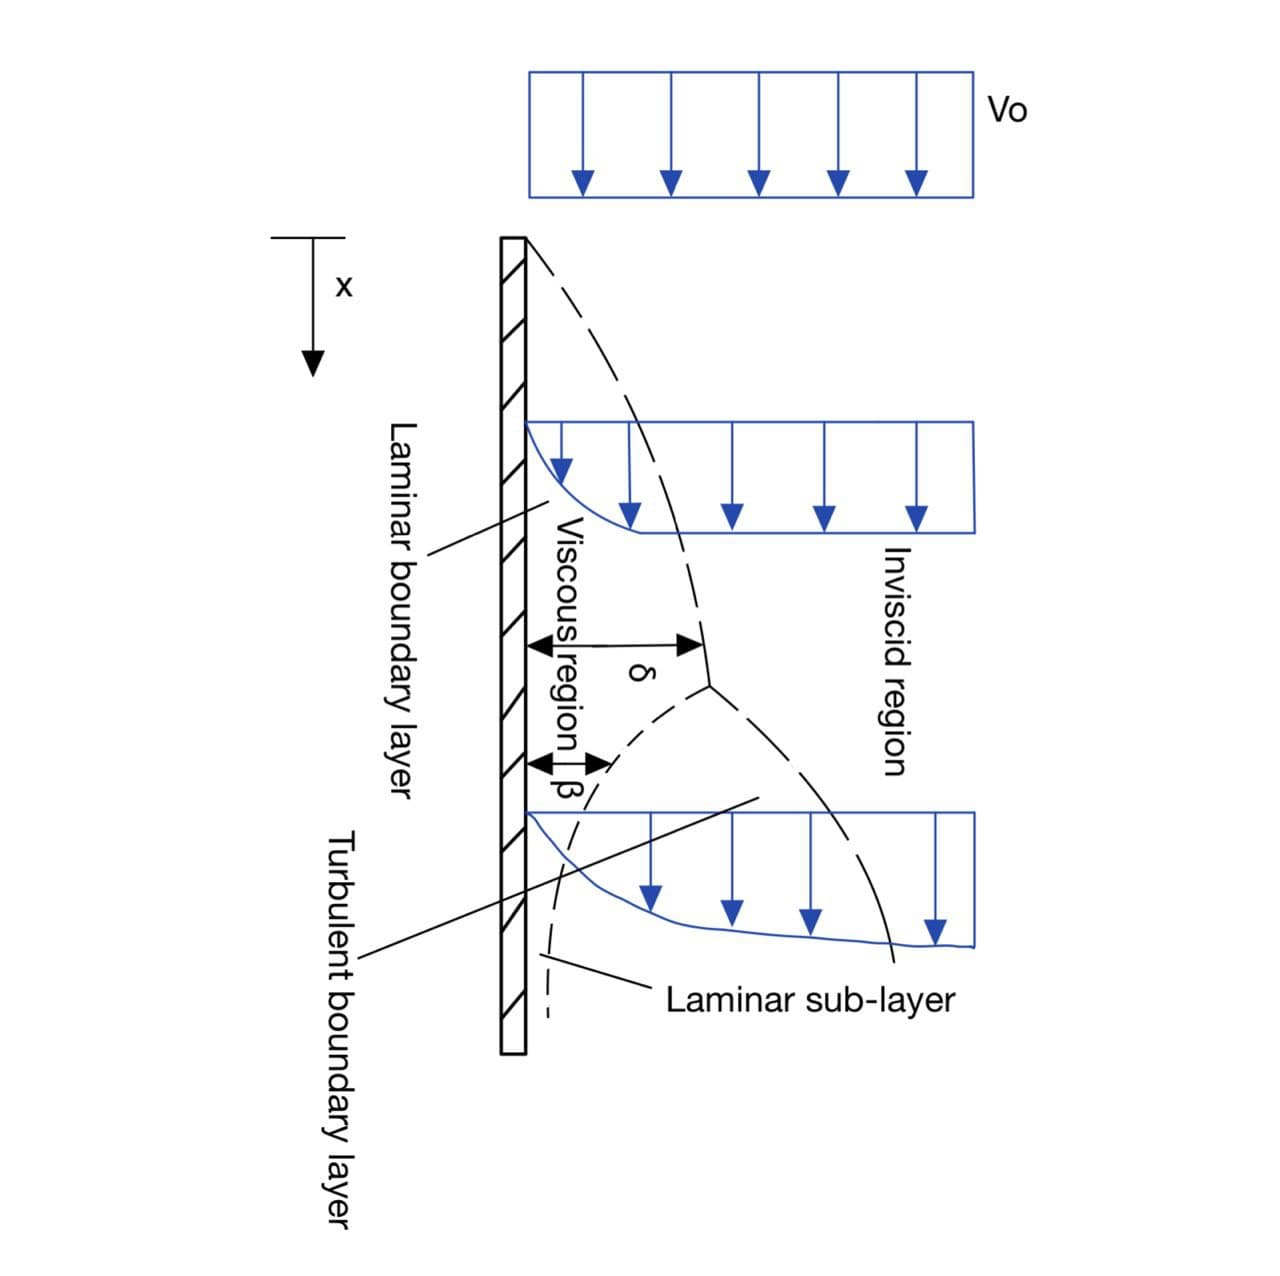
\includegraphics[width=0.65\textwidth]{PICTURES/BL.jpg}
    \caption{Boundary layer}
    \label{fig:BL}       % Give a unique label
\end{figure}

According to Prandtl's Boundary layer theory \cite{anderson2005ludwig}, 
\begin{equation}\label{eq:BL}
    \begin{aligned} \delta &\approx \begin{cases}\begin{aligned}
        &\frac{5.0x}{{Re^{1/2}}_x} &\textrm{laminar} \\ \\
        &\frac{0.16x}{{Re^{1/7}}_x} &\textrm{turbulent}\\
    \end{aligned}\end{cases}
\end{aligned}
\end{equation}
Reynolds number for the flow field along the wall:
\begin{equation}
Re_x = \frac{v_0x}{\nu} \\
\end{equation}

Reynolds number for open-channel flow \cite{french1985open}:
\begin{equation}
\begin{aligned} 
        Re_x & < 500 &\textrm{laminar} \\
        Re_x & > 12500 &\textrm{turbulent} \\
    \end{aligned}
\end{equation}

For the velocities 1mm/min, 0.5mm/min and 5mm/min, maximum wall length($x$) of 15mm, and kinematic viscosity($\nu$) of 
water at 10$^\circ$C 1.3063e-6[$m^2/s$] \cite{wagner2008iapws} boundary layer thickness was calculated using \cref{eq:BL}. 
Boundary layer thickness at the end of the wall for flow-velocity 1mm/min was calculated approximately equal to 170mm; 
for flow-velocity 5mm/min, it was 75mm; and for flow-velocity 0.5mm/min, it was 240mm. As discussed in the chapter 
\ref{chapter:modelconcept}, subsection \ref{ssec:impdum}, we chose small domain because of the local Newton solver we 
implemented had a restriction in the max time step size to be small which restricted running the simulation for longer times 
and for bigger domains -- otherwise, CPU time for running the simulation would be too high. The scope of the study was limited to 
implement chemical kinetics and its coupling with the freeflow Navier-Stokes model, so it wasn't a matter of paramount importance. 
In order to run the simulation for a longer time -- time for the solution to reach steady-state -- we had to shrink the domain size 
(we chose 5mm $\times$ 15mm). The width of the domain in x-direction is just 5mm compared to the boundary layer thicknesses; we were essentially 
inside the viscous region. Hence, mathematically, we should not see any difference between with and without grid grading near the wall, but we 
would also like to see if the model in \DuMuX is consistent with the mathematical calculation -- which is why we set the grid grading scenarios 
near the reactive wall as shown in \cref{fig:BL}. \\

\section{\DuMuX Simulation results}

\subsection{\DuMuX Simulation results: Open system}

\subsubsection*{Different flow velocities}\label{ssec:diffFlowVel}
We set the initial pH of the water to 6 and varied the flow velocity, but did not include grid grading parameters in the input file. We set the initial concentration of \ce{CO2} throughout the domain to be 2.5e-7 [mol\_\ce{CO2}/mol\_\ce{H2O}] and the boundary condition at the top of the domain to be 9.9956e-4 [mol/mol].
%% cite the source to use these concentrations


\begin{figure}[!h]
        \centering
    \begin{subfigure}{.5\linewidth}
        \centering
        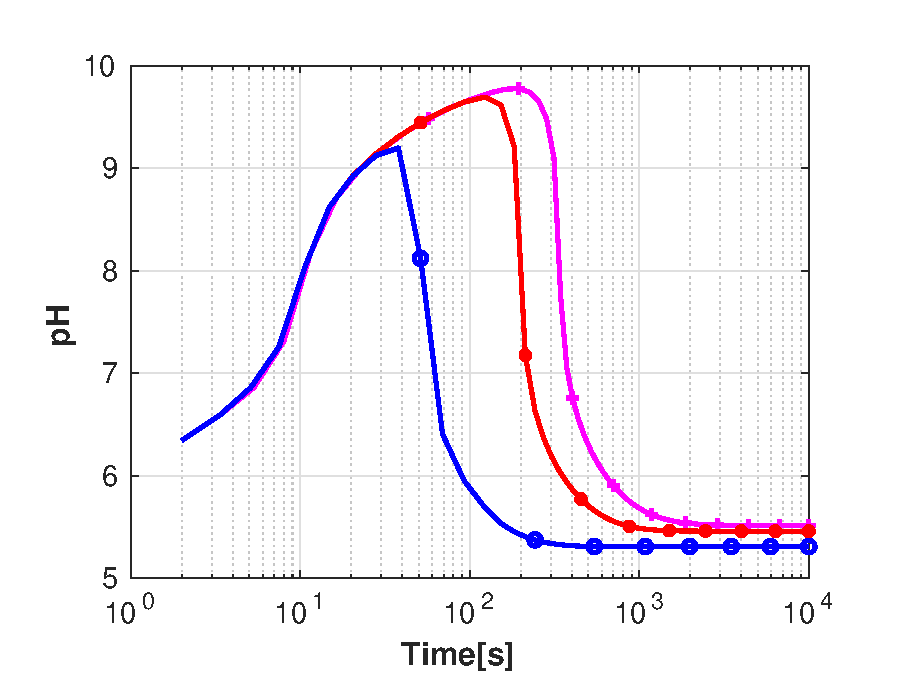
\includegraphics[width=\textwidth]{PICTURES/with_vel_pH.eps}
        \caption{Change in pH}
        \label{fig:velpH}       % Give a unique label
    \end{subfigure}%
        \hfill
        % here was an empty line which caused that the plots where not next
        % to each other but on top of each other
    \begin{subfigure}{.5\linewidth}
        \centering
        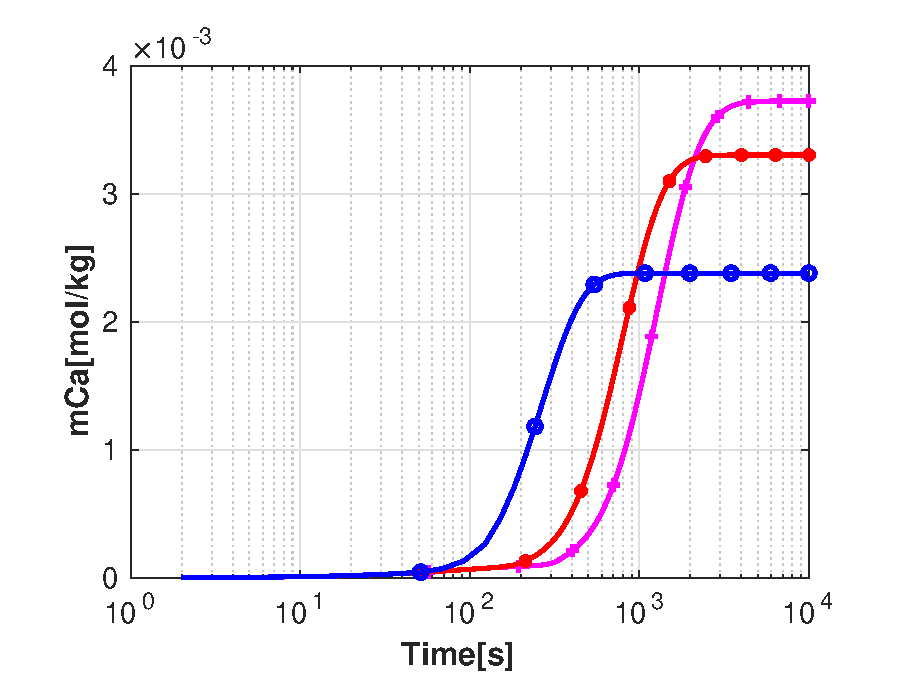
\includegraphics[width=\textwidth]{PICTURES/with_vel_mCa.eps}
        \caption{Change in molality of calcium (mCa)}
        \label{fig:velmCa}       % Give a unique label
    \end{subfigure}%
        \hfill
    \begin{subfigure}{.5\linewidth}
        \centering
        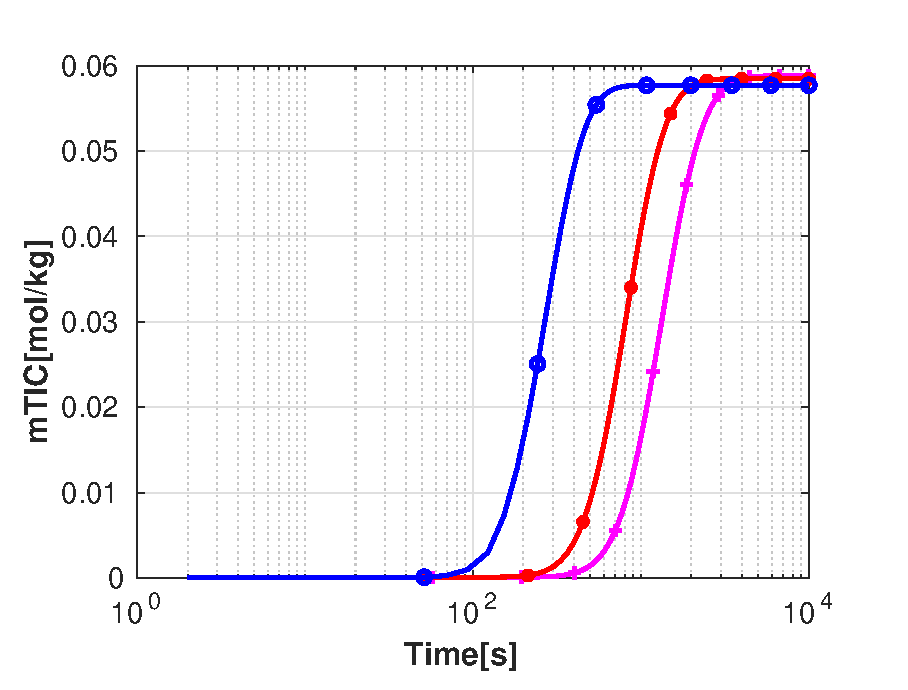
\includegraphics[width=\textwidth]{PICTURES/with_vel_mTIC.eps}
        \caption{Change in molality of total inorganic carbon (mTIC)}
        \label{fig:velmTIC}
    \end{subfigure}%
    \hfill
    \begin{subfigure}{.5\linewidth}
        \centering
        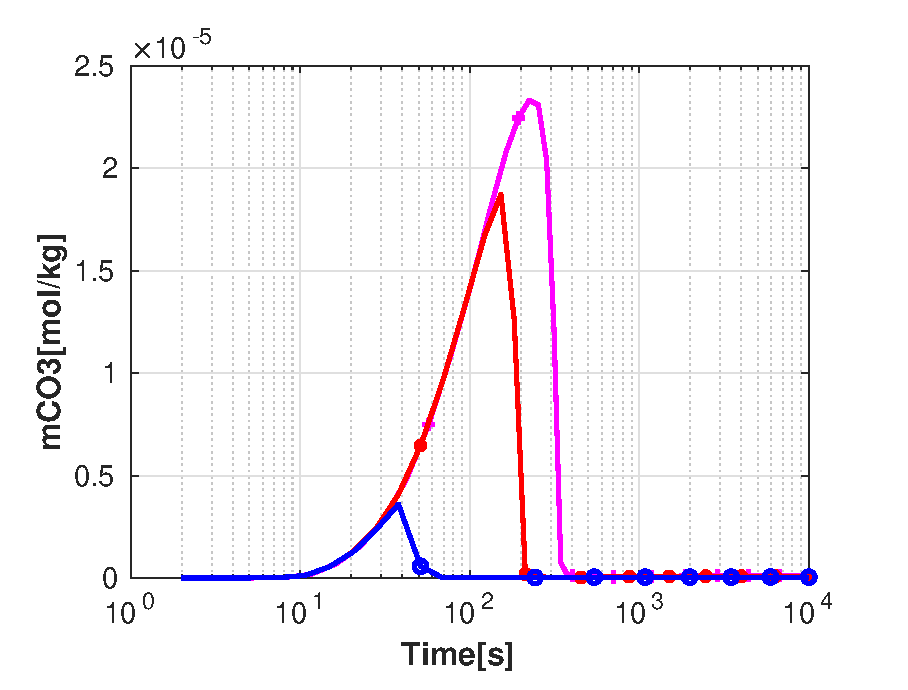
\includegraphics[width=\textwidth]{PICTURES/with_vel_mCO3.eps}
        \caption{Change in molality of carbonate (mCO3)}
        \label{fig:velmCO3}
    \end{subfigure}%
    \hfill
    \begin{subfigure}{.5\linewidth}
        \centering
        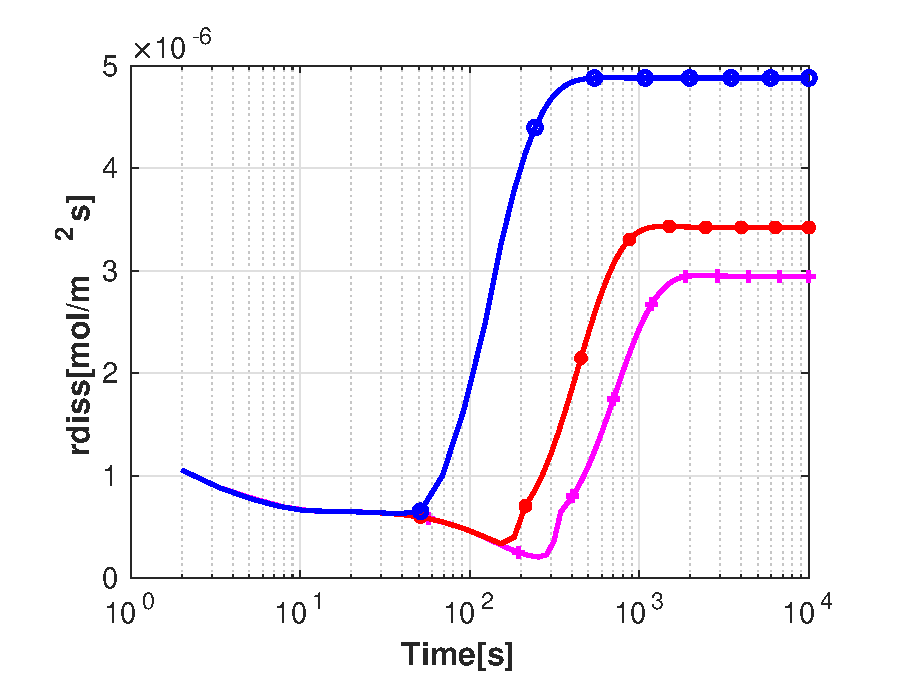
\includegraphics[width=\textwidth]{PICTURES/with_vel_rdiss.eps}
        \caption{Change in rate of dissolution of calcite (rdiss)}
        \label{fig:velrdiss}
    \end{subfigure}%
    \begin{subfigure}{.5\linewidth}
        \centering
        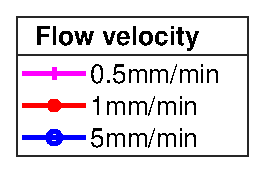
\includegraphics[width=0.40\textwidth]{PICTURES/with_vel_legend.eps}
        \caption{Legend}
        \label{fig:vellegend}
    \end{subfigure}%
    \hfill
     \caption{\DuMuX results that show the change in pH (\cref{fig:velpH}), molality of calcium (\cref{fig:velmCa}), 
     molality of total inorganic carbon (\cref{fig:velmTIC}), molality of carbonate (\cref{fig:velmCO3}) and rate of 
     dissolution of calcite (\cref{fig:velrdiss}) in time for different flow velocities in an open system}
     \label{fig:comparisionDiffFlowVelocity}
\end{figure}

The plots shown in figure \ref{fig:comparisionDiffFlowVelocity} is obtained for a cell at the boundary wall. 
All of the subplots, i.e., \subref{fig:1mmpermin}, \subref{fig:5mmpermin} and \subref{fig:0.5mmpermin}, 
show pH rises over time, reaches to its peak, and then descends to a steady-state value. The peak value 
varies with different initial and boundary conditions setups. 
The initial concentration of \code{TIC} i.e. 2.5e-7 [mol/mol] in the system is lower than the 
boundary condition i.e. 9.9956e-4 [mol/mol]. This leads to a low buffering capacity of the solution at the 
beginning, and with the incoming \ce{CO2} having higher concentration, pH rises rapidly. As time passes, 
the dissolved calcium-carbonate is transported away from the system and hence pH lowers and reaches a steady-state value.\\
Considering all the parameters to be constant, with the increase in flow-velocity the maximum pH decreases and system stabilizes faster. 
The reason is with faster transport of increased TIC, which is due to additional \ce{CO2} transported into the system and 
dissolved calcium-carbonate because of the reaction at the wall, out of the system due to higher flow velocity. 
Had there been initial and boundary conditions, we would not expect this peak to occur. It is because of the inconsistent 
BCs with the initial conditions that lead to this phenomenon. Since, we are mainly checking the plausibility of the model, 
we did not consider in defining a consistent BCs and initial conditions. A detail explanation to this phenomena and its dependency 
on initial and boundary conditions are discussed in subsection \ref{ssec:diffInitialBC}.


\subsubsection*{Different initial pH} \label{ssec:diffpH}
We fixed the flow-velocity to 1mm/min, did not include grid grading parameters, initial \ce{CO2} concentration was fixed to 2.5e-7[mol/mol] and boundary concentration at the top was set to 9.9956e-4[mol/mol]; just the initial pH at the start of the simulation were varied.

\begin{figure}[!h]
        \centering
    \begin{subfigure}{.5\linewidth}
            \centering
        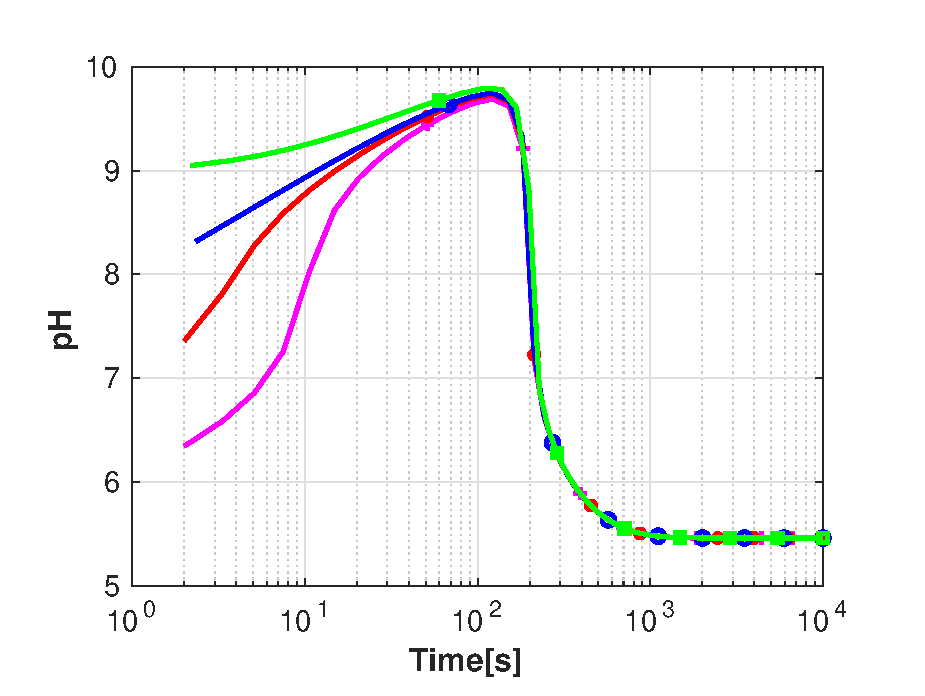
\includegraphics[width=\textwidth]{PICTURES/with_pH_pH.eps}
        \caption{Change in pH}
        \label{fig:pHpH}
    \end{subfigure}%
        \hfill
    \begin{subfigure}{.5\linewidth}
            \centering
        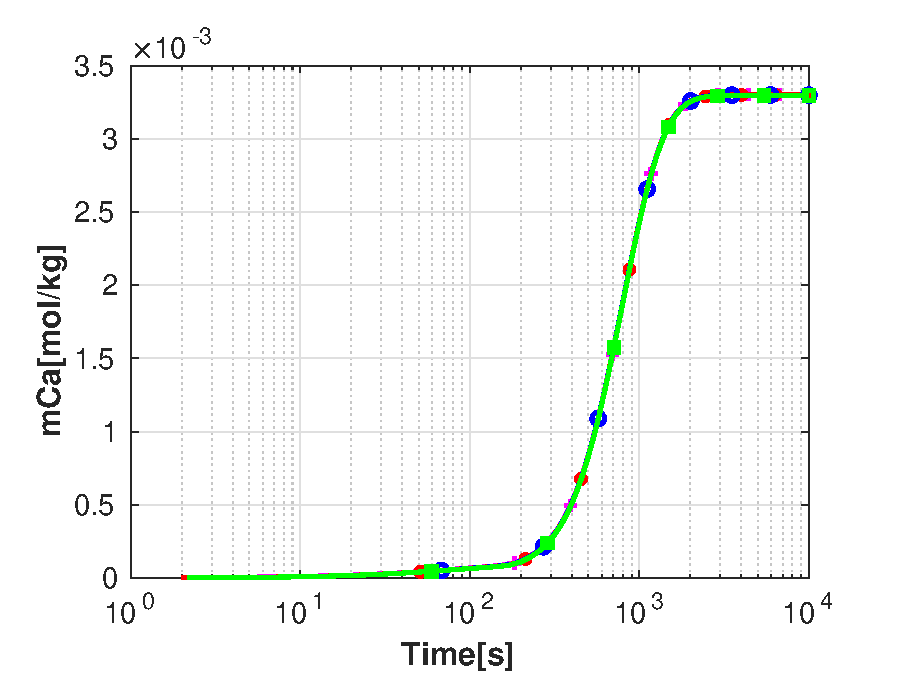
\includegraphics[width=\textwidth]{PICTURES/with_pH_mCa.eps}
        \caption{Change in molality of calcium (mCa)}
        \label{fig:pHmCa}
    \end{subfigure}%
    \hfill
    \begin{subfigure}{.5\linewidth}
            \centering
        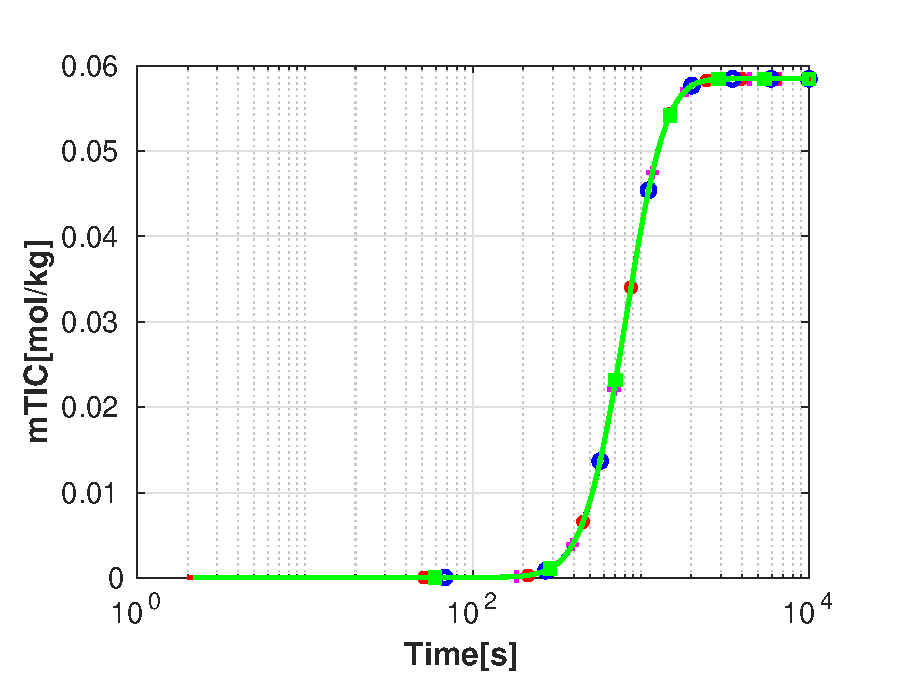
\includegraphics[width=\textwidth]{PICTURES/with_pH_mTIC.eps}
        \caption{Change in molality of total inorganic carbon (mTIC)}
        \label{fig:pHmTIC}
    \end{subfigure}%
    \hfill
    \begin{subfigure}{.5\linewidth}
            \centering
        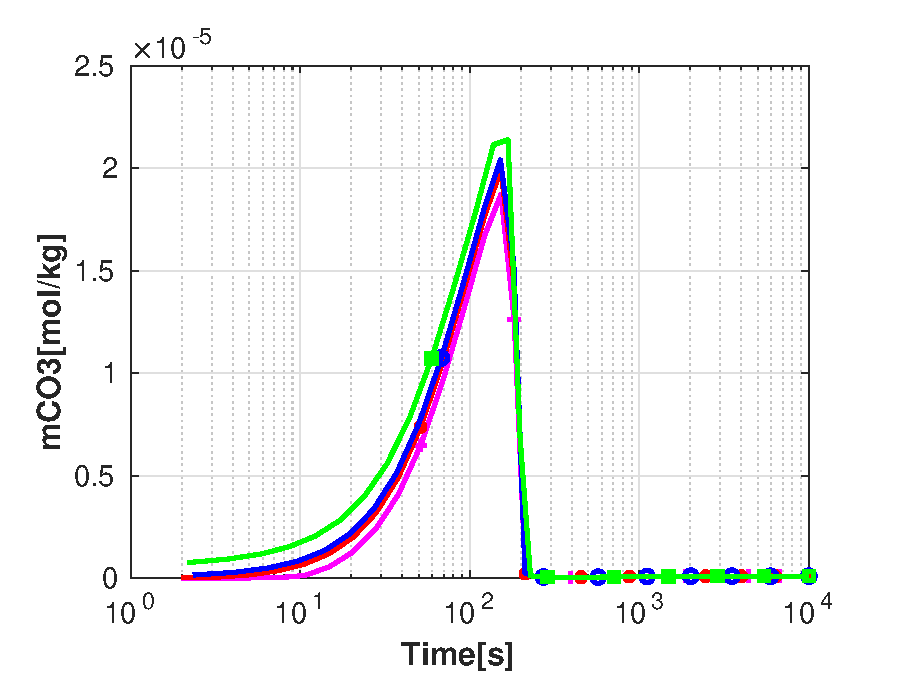
\includegraphics[width=\textwidth]{PICTURES/with_pH_mCO3.eps}
        \caption{Change in molality of carbonate (mCO3)}
        \label{fig:pHmCO3}
    \end{subfigure}%
    \hfill
    \begin{subfigure}{.5\linewidth}
            \centering
        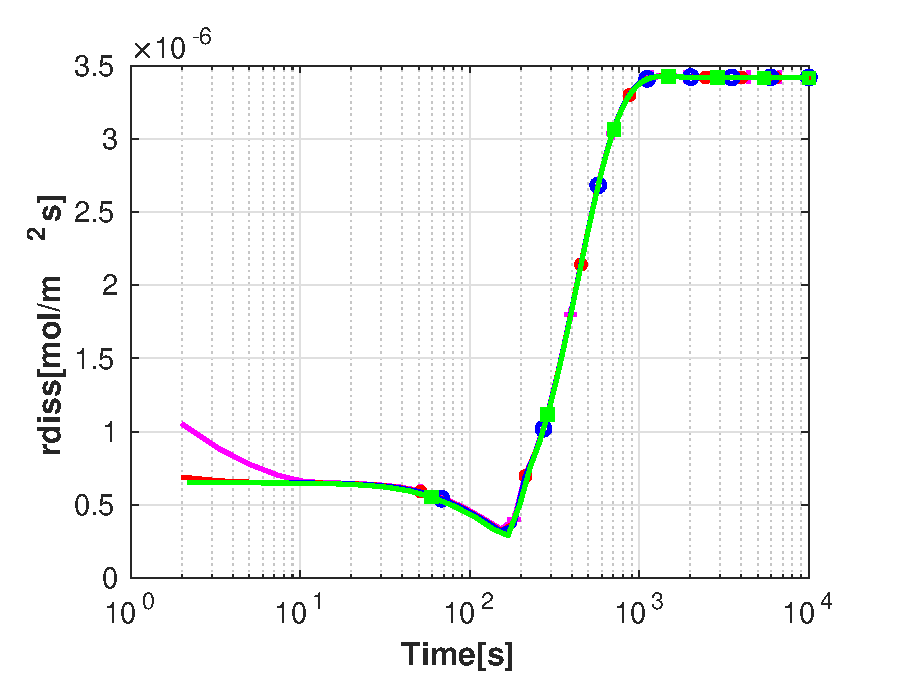
\includegraphics[width=\textwidth]{PICTURES/with_pH_rdiss.eps}
        \caption{Change in rate of dissolution of calcite (rdiss)}
        \label{fig:pHrdiss}
    \end{subfigure}%
  \hfill
  \begin{subfigure}{.5\linewidth}
            \centering
        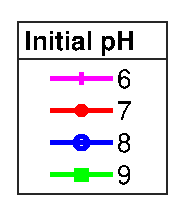
\includegraphics[width=0.25\textwidth]{PICTURES/with_pH_legend.eps}
        \caption{Legend}
        \label{fig:pHlegend}
    \end{subfigure}%
    \caption{\DuMuX results that show the change in pH (\cref{fig:pHpH}), molality of calcium (\cref{fig:pHmCa}), 
    molality of total inorganic carbon (\cref{fig:pHmTIC}), molality of carbonate (\cref{fig:pHmCO3}) and rate of 
    dissolution of calcite (\cref{fig:pHrdiss}) in time for different initial pH in an open system}
    \label{fig:comparisionDiffInitialpH}
\end{figure}


The figure \ref{fig:comparisionDiffInitialpH} shows pH rises over time, reaches to its peak, and then descends to a steady-state value, as seen on figure \ref{fig:comparisionDiffFlowVelocity}. The explanation for such phenomena holds true here as well. Increasing the initial pH also increases the steady-state pH. The time for system to be in steady-state is fairly same for all the cases, as expected. Since, this depends on the flow-velocity and initial and boundary concentration of \ce{CO2}, which is constant for all the cases. 

\subsubsection*{Different initial and boundary \ce{CO2} concentrations} \label{ssec:diffInitialBC}
We fixed the flow-velocity to 1mm/min, did not include grid grading and initial pH was set to 6.0; just the boundary condition at the top of the domain was varied to analyse the buffering effect in the pH growth of the water, keeping a constant initial concentration of \ce{CO2} inside the domain to be 2.5e-7 [mol/mol].

\begin{figure}[!h]
        \centering
    \begin{subfigure}{.5\linewidth}
            \centering
        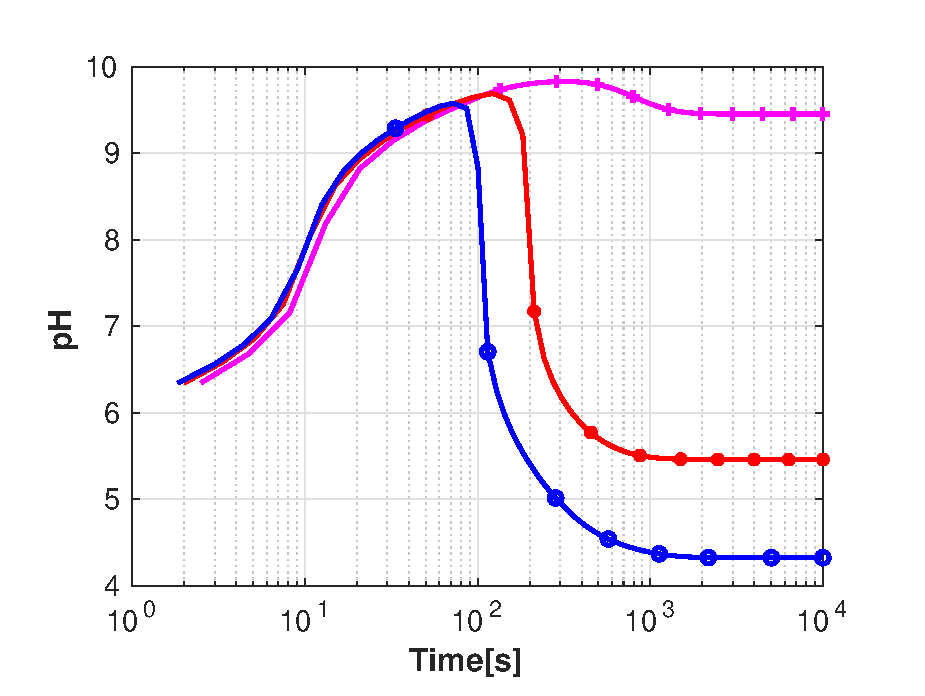
\includegraphics[width=\textwidth]{PICTURES/with_CO2_pH.eps}
        \caption{Change in pH}
        \label{fig:CO2pH}
    \end{subfigure}%
        \hfill
    \begin{subfigure}{.5\linewidth}
            \centering
        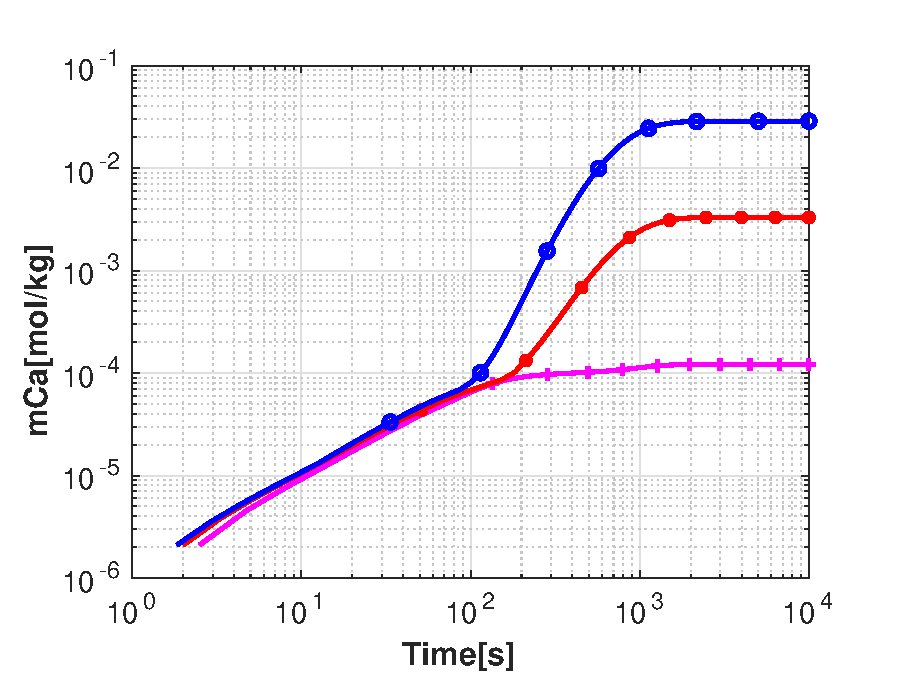
\includegraphics[width=\textwidth]{PICTURES/with_CO2_mCa.eps}
        \caption{Change in molality of calcium (mCa)}
        \label{fig:CO2mCa}
    \end{subfigure}%
        \hfill
    \begin{subfigure}{.5\linewidth}
            \centering
        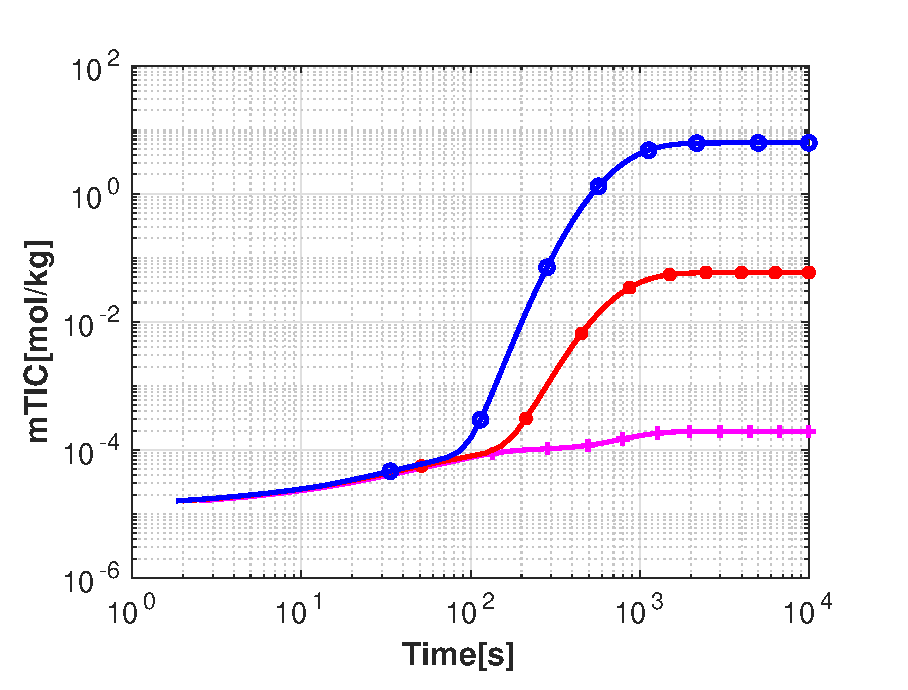
\includegraphics[width=\textwidth]{PICTURES/with_CO2_mTIC.eps}
        \caption{Change in molality of total inorganic carbon (mTIC)}
        \label{fig:CO2mTIC}
    \end{subfigure}%
    \hfill
    \begin{subfigure}{.5\linewidth}
            \centering
        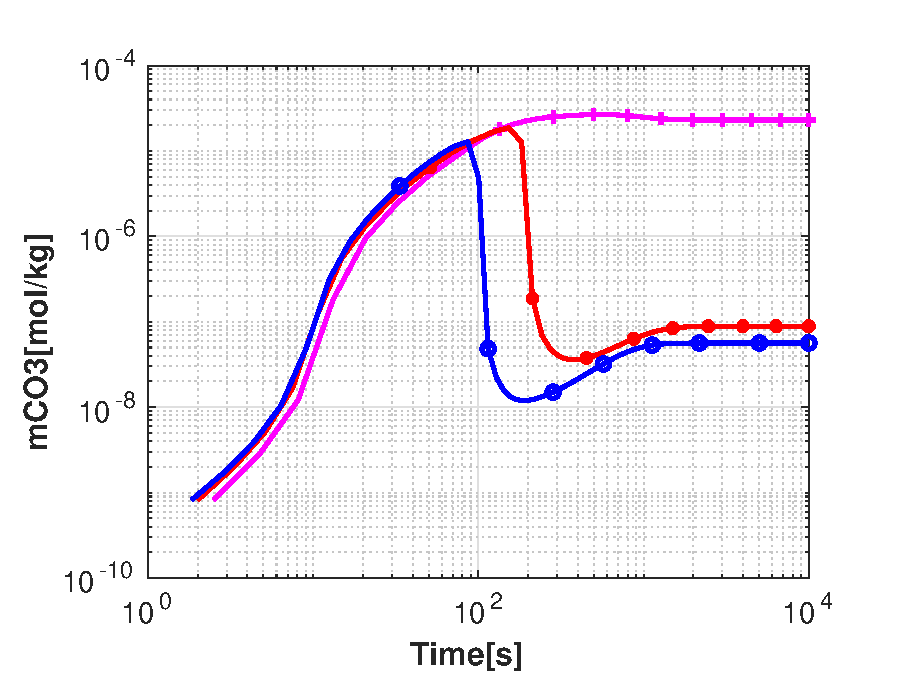
\includegraphics[width=\textwidth]{PICTURES/with_CO2_mCO3.eps}
        \caption{Change in molality of carbonate (mCO3)}
        \label{fig:CO2mCO3}
    \end{subfigure}%
    \hfill
    \begin{subfigure}{.5\linewidth}
            \centering
        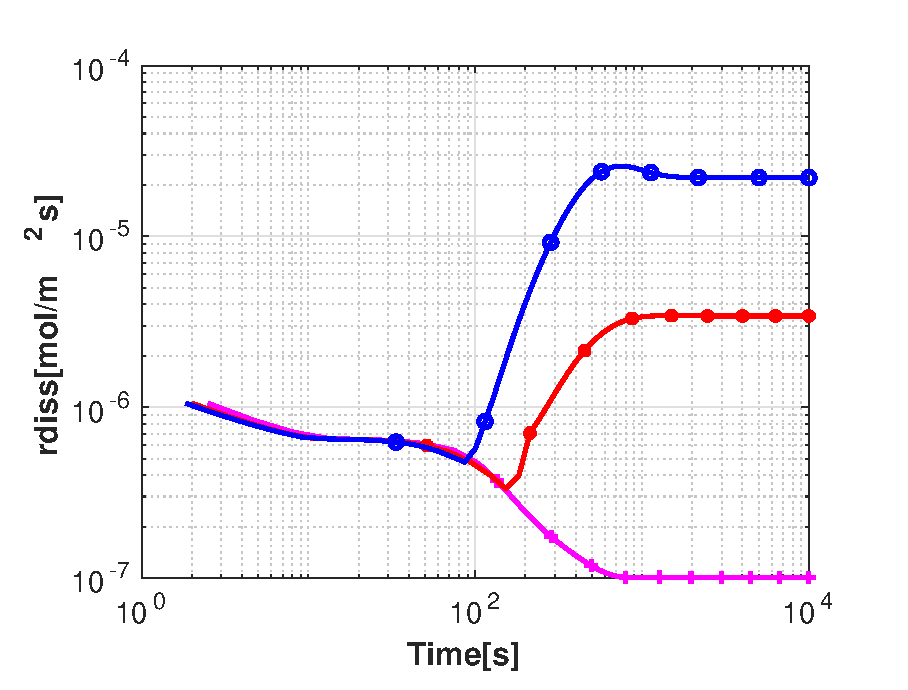
\includegraphics[width=\textwidth]{PICTURES/with_CO2_rdiss.eps}
        \caption{Change in rate of dissolution of calcite (rdiss)}
        \label{fig:CO2rdiss}
    \end{subfigure}%
    \hfill
    \begin{subfigure}{.5\linewidth}
            \centering
        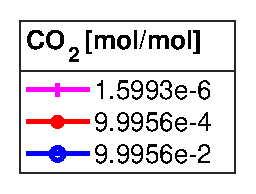
\includegraphics[width=0.35\textwidth]{PICTURES/with_CO2_legend.eps}
        \caption{Legend}
        \label{fig:CO2legend}
    \end{subfigure}%
    \caption{\DuMuX results that show the change in pH (\cref{fig:CO2pH}), molality of calcium (\cref{fig:CO2mCa}), molality of total inorganic carbon (\cref{fig:CO2mTIC}), molality of carbonate (\cref{fig:CO2mCO3}) and rate of dissolution of calcite (\cref{fig:CO2rdiss}) in time for different \ce{CO2} concentration at the top of the domain in an open system}
    \label{fig:diffCO2}
\end{figure}

The figure \ref{fig:diffCO2} shows the same rise in pH, with same pattern, over time. The difference now is the maximum pH and the steady-state pH value; the steady-state time is once again similar for all the subplots in fig. \ref{fig:CO2}. Decreasing the \ce{CO2} concentration at the top, but it still has a higher \ce{CO2} concentration than what's inside, as shown in fig. \subref{fig:CO2low}, shows the system is more or less consistent with the inside and incoming \ce{CO2}-enriched water. The pH rises steadily and reaches a peak, and without descending, stabilizes around same steady-state value. The dissolution capacity of water has not changed much throughout the simulation.\\
On the other hand, figure \subref{fig:CO2high} shows the same pattern as in figure \ref{fig:CO2} with a different peak and steady-state pH. The incoming water has higher \ce{CO2} concentration which mixes/replaces the lower \ce{CO2}-enriched water. Because of \ce{CO2}, reaction advances and hence pH rises, but as the simulation proceeds, the lower \ce{CO2}-enriched water with low buffering capacity is being replaced by water with high buffering capacity. Hence, the rise in pH is subdued and the pH falls until it reaches steady-state. 


\subsubsection*{Different Grid grading parameter} \label{ssec:diffGrid}
We fixed the initial pH to 6.0, flow-velocity to 1mm/min, initial \ce{CO2} was fixed to 2.5e-7[mol/mol] and at the boundary it was 9.9956e-4[mol/mol]; just the grid grading parameter was varied to properly resolve the boundary layer formation on the wall. We expect a boundary layer formation on the reactive wall in a cave scenario, but given the size of the domain we have, we were not able to see any difference in output values with and without grid-grading parameters. \\
We decreased the spacing of the grids near the wall in x-direction. We ran the simulation for grid-grading values 1.1 and 1.2.

\begin{figure}[!h]
        \centering
    \begin{subfigure}{.5\linewidth}
            \centering
        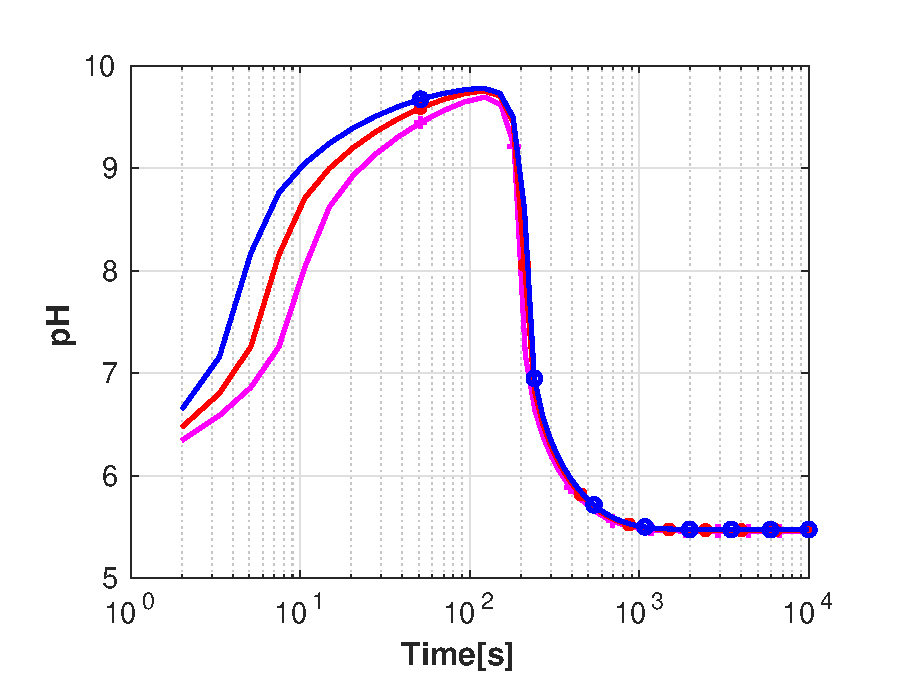
\includegraphics[width=\textwidth]{PICTURES/with_grid_pH.eps}
        \caption{Change in pH}
        \label{fig:gridpH}
    \end{subfigure}%
        \hfill
    \begin{subfigure}{.5\linewidth}
            \centering
        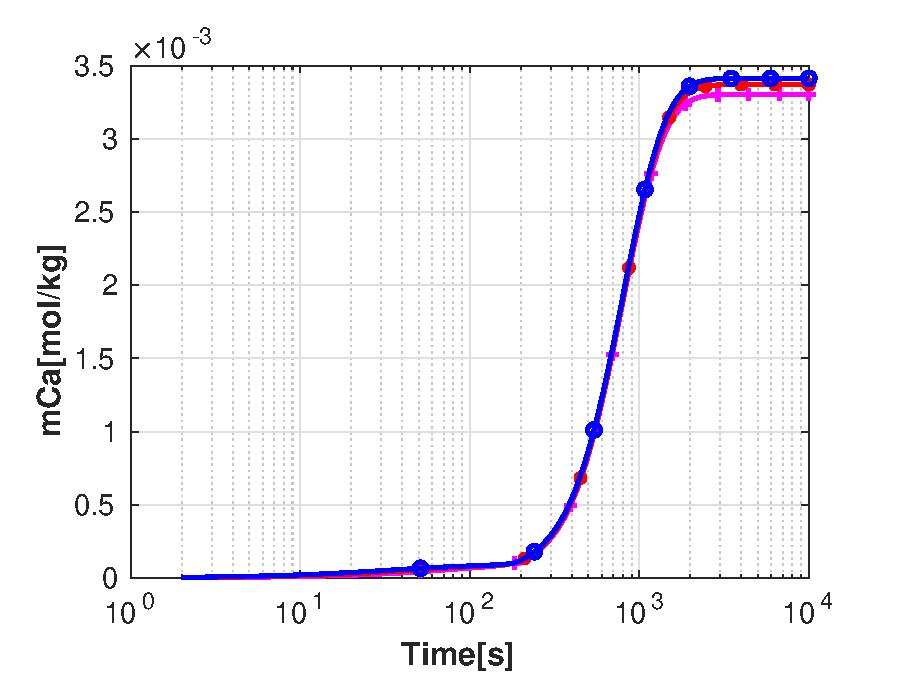
\includegraphics[width=\textwidth]{PICTURES/with_grid_mCa.eps}
        \caption{Change in molality of calcium (mCa)}
        \label{fig:gridmCa}
    \end{subfigure}%
        \hfill
        \begin{subfigure}{.5\linewidth}
            \centering
        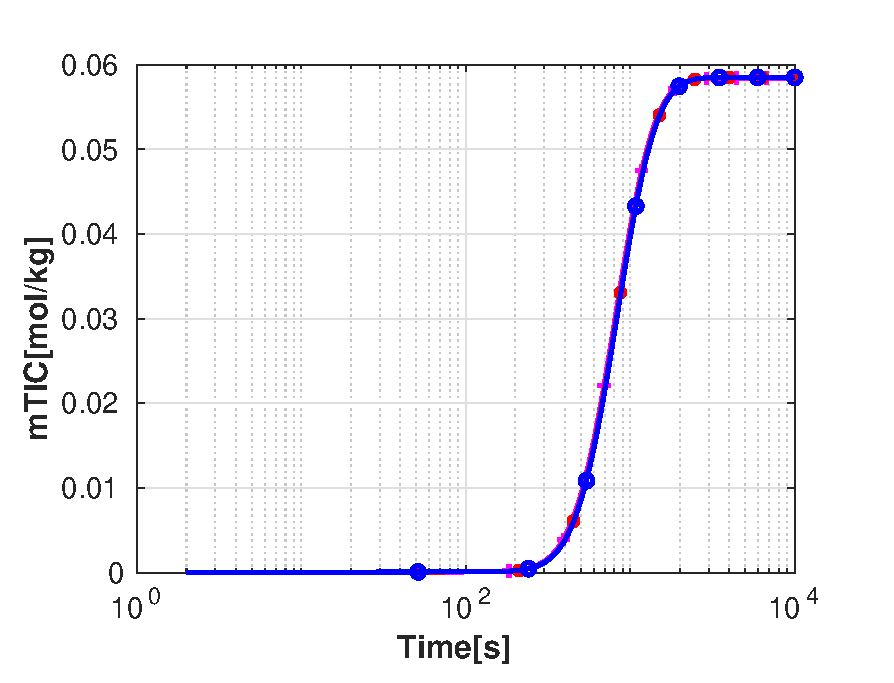
\includegraphics[width=\textwidth]{PICTURES/with_grid_mTIC.eps}
        \caption{Change in molality of total inorganic carbon (mTIC)}
        \label{fig:gridmTIC}
    \end{subfigure}%
        \hfill
        \begin{subfigure}{.5\linewidth}
            \centering
        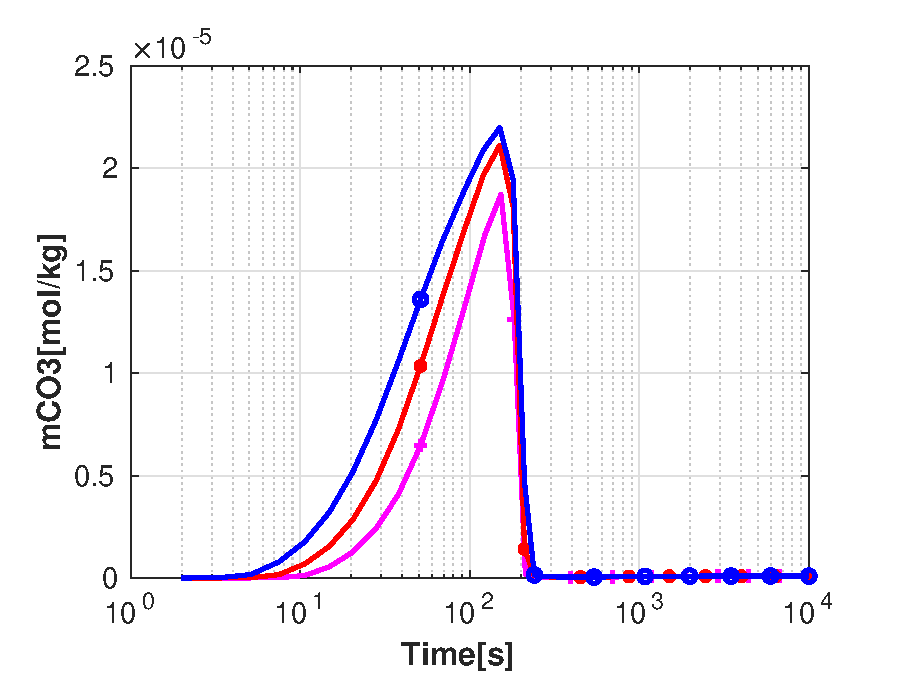
\includegraphics[width=\textwidth]{PICTURES/with_grid_mCO3.eps}
        \caption{Change in molality of carbonate (mCO3)}
        \label{fig:gridmCO3}
    \end{subfigure}%
        \hfill
        \begin{subfigure}{.5\linewidth}
            \centering
        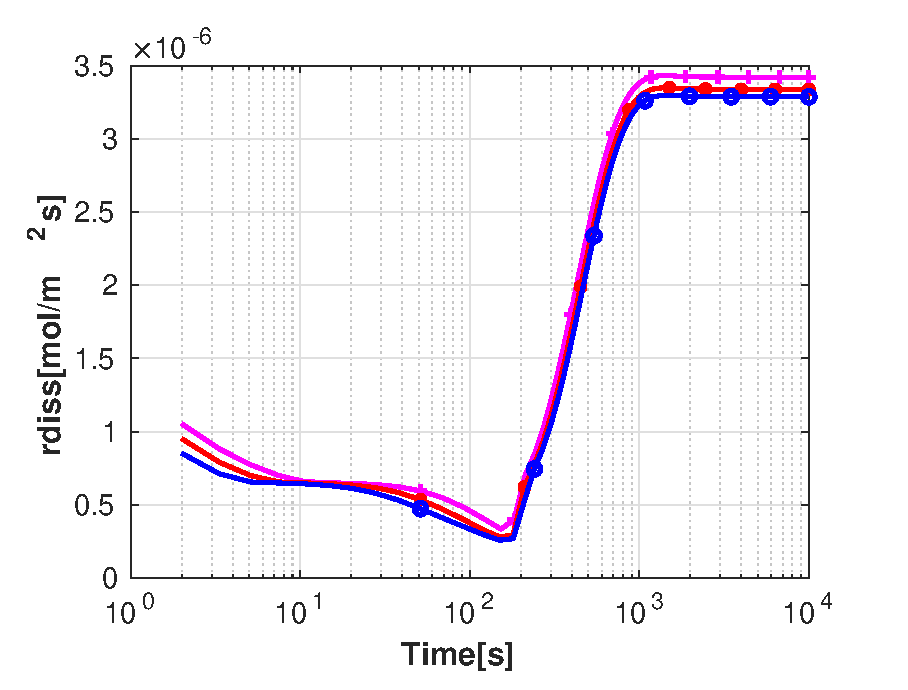
\includegraphics[width=\textwidth]{PICTURES/with_grid_rdiss.eps}
        \caption{Change in rate of dissolution of calcite (rdiss)}
        \label{fig:gridrdiss}
    \end{subfigure}%
        \hfill
        \begin{subfigure}{.5\linewidth}
            \centering
        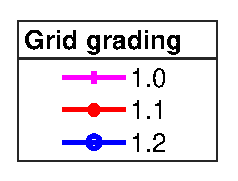
\includegraphics[width=0.35\textwidth]{PICTURES/with_grid_legend.eps}
        \caption{Legend}
        \label{fig:gridlegend}
    \end{subfigure}%
    \caption{\DuMuX results that show the change in pH (\cref{fig:gridpH}), molality of calcium (\cref{fig:gridmCa}), molality of total inorganic carbon (\cref{fig:gridmTIC}), molality of carbonate (\cref{fig:gridmCO3}) and rate of dissolution of calcite (\cref{fig:gridrdiss}) in time for different grid grading parameter in an open system}
    \label{fig:diffGrid}
\end{figure}

The reason we chose grid grading near the wall is to resolve the boundary layer developed on the wall. Since the model we chose was too small, we were inside the boundary layer and that was the reason why we did not see any differences in the subplots in the figure \ref{fig:diffGrid}.

\subsubsection*{Contour plots} \label{ssec:contour}
We fixed pH of the water to 6 and did not include grid grading parameters in the input file -- just the flow velocity was varied. We set the initial concentration of \ce{CO2} throughout the domain to be 2.5e-7 [mol\_\ce{CO2}/mol\_\ce{H2O}] and the boundary condition at the top of the domain to be 9.9956e-4 [mol/mol].


\paragraph*{pH contour plots} \mbox{}\\
% steady state pH
\begin{figure}[!h]
\centering
    \begin{subfigure}{.5\linewidth}
        \centering
        \includegraphics[trim=450 20 450 20, clip, width=0.9\textwidth]{PICTURES/contour_vel1mm_pH.eps}
        \caption{Flow Velocity = 1mm/min}
        \label{fig:pHSteady-state}       % Give a unique label
    \end{subfigure}%
    \hfill
    \begin{subfigure}{.5\linewidth}
        \centering
        \includegraphics[trim=450 20 450 20, clip, width=0.9\textwidth]{PICTURES/contour_vel5mm_pH.eps}
        \caption{Flow Velocity = 5mm/min}
        \label{fig:pHSteady-state5mm}       % Give a unique label
    \end{subfigure}%
    \hfill
    \begin{subfigure}{.5\linewidth}
        \centering
        \includegraphics[trim=450 20 450 20, clip, width=\textwidth]{PICTURES/contour_vel0.5mm_pH.eps}
        \caption{Flow Velocity = 0.5mm/min}
        \label{fig:pHSteady-state0.5mm}       % Give a unique label
    \end{subfigure}%
    \caption{\DuMuX Contour plots: Numerical results that show the distribution of pH at the steady-state in an open system}
     \label{fig:contourpH}
\end{figure}

Figure \ref{fig:contourpH} shows contour plots for pH at the steady-state in varying flow-velocities. All the subplots \ref{fig:pHSteady-state}, \ref{fig:pHSteady-state5mm}, \ref{fig:pHSteady-state0.5mm} show higher pH value near the reactive wall, and the pH decreases as we go away from the wall. The dissolved calcium-carbonate is diffused along the x-axis which causes the rise in pH adjacent to the reactive wall which fades out as we go away from the wall.


\paragraph*{mCO3 contour plots} \mbox{}\\

%steady-state CO3
\begin{figure}[!h]
\centering
    \begin{subfigure}{.5\linewidth}
        \centering
        \includegraphics[trim=450 20 450 20, clip, width=0.9\textwidth]{PICTURES/contour_vel1mm_mCO3.eps}
        \caption{Flow Velocity = 1mm/min}
        \label{fig:CO3Steady-state}       % Give a unique label
    \end{subfigure}%
    \hfill
    \begin{subfigure}{.5\linewidth}
        \centering
        \includegraphics[trim=450 20 450 20, clip, width=0.9\textwidth]{PICTURES/contour_vel5mm_mCO3.eps}
        \caption{Flow Velocity = 5mm/min}
        \label{fig:CO3Steady-state5mm}       % Give a unique label
    \end{subfigure}%
    \hfill
    \begin{subfigure}{.5\linewidth}
        \centering
        \includegraphics[trim=450 20 450 20, clip, width=0.9\textwidth]{PICTURES/contour_vel0.5mm_mCO3.eps}
        \caption{Flow Velocity = 0.5mm/min}
        \label{fig:CO3Steady-state0.5mm}       % Give a unique label
    \end{subfigure}%
    \caption{\DuMuX Contour plots: Numerical results that show the distribution of molality of carbonate at the steady-state in an open system}
     \label{fig:contourCO3}
\end{figure}


Figure \ref{fig:contourCO3} shows contour plots for the concentration of \ce{CO3}\textsuperscript{2-} at the steady-state in varying flow-velocities. All the subplots \ref{fig:CO3Steady-state}, \ref{fig:CO3Steady-state5mm}, \ref{fig:CO3Steady-state0.5mm} show a similar pattern: higher concentration near the reactive wall, where dissolution of calcium-carbonate is adding \ce{CO3}\textsuperscript{2-} into the karst water. As we go away from the wall, concentration of \ce{CO3}\textsuperscript{2-} starts to decrease -- the dissolved calcium-carbonate is diffused along the x-axis which causes a formation of concentration gradient along x-axis -- and reaches as far as the diffusion takes it. Had the simulation ran for longer times than for 6000s (the time we ran for this case), the contour would have migrated further to the right. 

\paragraph*{mTIC contour plots} \mbox{}\\
% steady state TIC
\begin{figure}[!h]
\centering
    \begin{subfigure}{.5\linewidth}
        \centering
        \includegraphics[trim=450 20 450 20, clip, width=0.9\textwidth]{PICTURES/contour_vel1mm_mTIC.eps}
        \caption{Flow Velocity = 1mm/min}
        \label{fig:TICSteady-state}       % Give a unique label
    \end{subfigure}%
    \hfill
    \begin{subfigure}{.5\linewidth}
        \centering
        \includegraphics[trim=450 20 450 20, clip, width=0.9\textwidth]{PICTURES/contour_vel5mm_mTIC.eps}
        \caption{Flow Velocity = 5mm/min}
        \label{fig:TICSteady-state5mm}       % Give a unique label
    \end{subfigure}%
    \hfill
    \begin{subfigure}{.5\linewidth}
        \centering
        \includegraphics[trim=450 20 450 20, clip, width=0.9\textwidth]{PICTURES/contour_vel0.5mm_mTIC.eps}
        \caption{Flow Velocity = 0.5mm/min}
        \label{fig:TICSteady-state0.5mm}       % Give a unique label
    \end{subfigure}%
    \caption{\DuMuX Contour plots: Numerical results that show the distribution of molality of total inorganic carbon at the steady-state in an open system}
     \label{fig:contourTIC}
\end{figure}

Figure \ref{fig:contourTIC} shows contour plots for concentration of Total Inorganic Carbon (TIC) at the steady-state in varying flow-velocities. All the subplots \ref{fig:TICSteady-state}, \ref{fig:TICSteady-state5mm}, \ref{fig:TICSteady-state0.5mm} show the system has more or less come to a steady-state. \ce{CO2} is carried into the system with the flow, which also gets diffused and gets mixed within the system as the time progresses, which causes the concentration to be fairly constant throughout the system. 


\paragraph*{mCa contour plots} \mbox{}\\

% steady state Ca
\begin{figure}[!h]
\centering
    \begin{subfigure}{.5\linewidth}
        \centering
        \includegraphics[trim=450 20 450 20, clip, width=0.9\textwidth]{PICTURES/contour_vel1mm_mCa.eps}
        \caption{Flow Velocity = 1mm/min}
        \label{fig:CaSteady-state}       % Give a unique label
    \end{subfigure}%
    \hfill
    \begin{subfigure}{.5\linewidth}
        \centering
        \includegraphics[trim=450 20 450 20, clip, width=0.9\textwidth]{PICTURES/contour_vel5mm_mCa.eps}
        \caption{Flow Velocity = 5mm/min}
        \label{fig:CaSteady-state5mm}       % Give a unique label
    \end{subfigure}%
    \hfill
    \begin{subfigure}{.5\linewidth}
        \centering
        \includegraphics[trim=450 20 450 20, clip, width=0.9\textwidth]{PICTURES/contour_vel0.5mm_mCa.eps}
        \caption{Flow Velocity = 0.5mm/min}
        \label{fig:CaSteady-state0.5mm}       % Give a unique label
    \end{subfigure}%
    \caption{\DuMuX Contour plots: Numerical results that show the distribution of molality of calcium at the steady-state in an open system}
     \label{fig:contourCa}
\end{figure}

Figure \ref{fig:contourCa} shows contour plots for concentration of Ca\textsuperscript{2+} at the steady-state in varying flow-velocities. All the subplots \ref{fig:CaSteady-state}, \ref{fig:CaSteady-state5mm}, \ref{fig:CaSteady-state0.5mm} show higher concentration near the reactive wall, and the concentration decreases as we go away from the wall. The dissolved calcium-carbonate is diffused along the x-axis which causes the rise in concentration of Ca\textsuperscript{2+} adjacent to the reactive wall which fades out as we go away from the wall.


\subsection{\DuMuX Simulation results: Closed system}
\subsubsection*{Different initial pH} \label{ssec:diffinitialpHnoflow}
The purpose of the simulation runs without flow-velocity was for the validation purpose with \MATLAB results. The initial concentration of \ce{CO2} in the karst water was set to 2.5e-7 [mol/mol]. We did not include grid grading parameters; the initial pH at the start of the simulation were varied.

\begin{figure}[!h]
        \centering
    \begin{subfigure}{.5\linewidth}
            \centering
        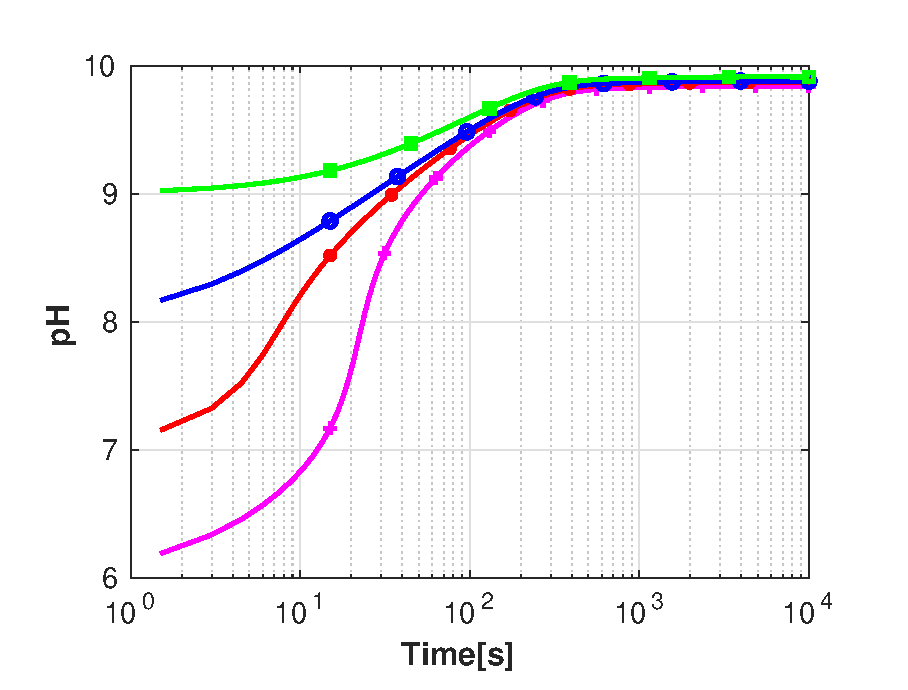
\includegraphics[width=\textwidth]{PICTURES/without_pH_pH.eps}
        \caption{Change in pH}
        \label{fig:withoutpHpH}
    \end{subfigure}%
        \hfill
    \begin{subfigure}{.5\linewidth}
            \centering
        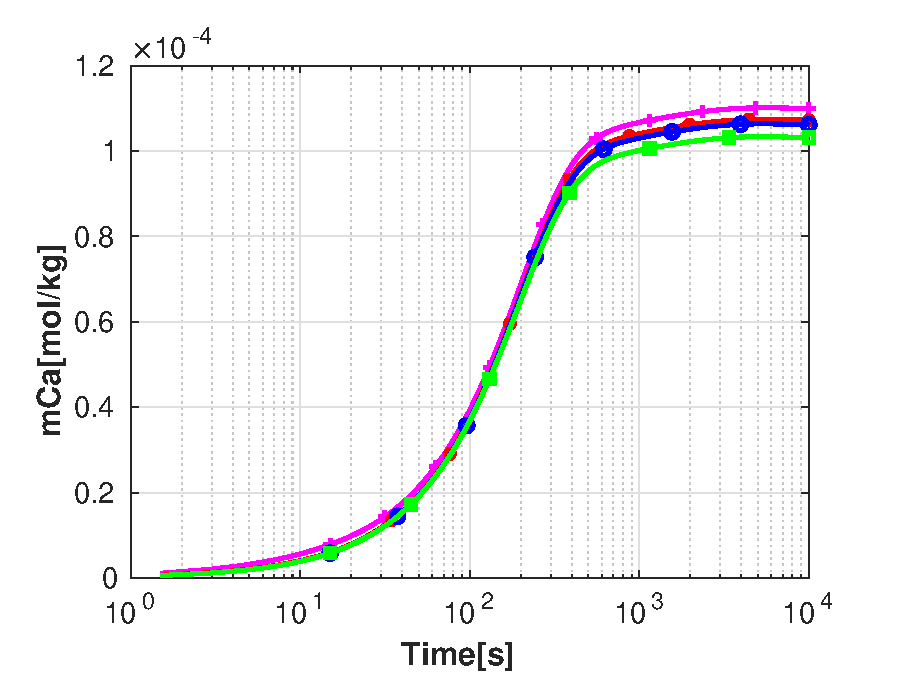
\includegraphics[width=\textwidth]{PICTURES/without_pH_mCa.eps}
        \caption{Change in molality of calcium (mCa)}
        \label{fig:withoutpHmCa}
    \end{subfigure}%
    \hfill
    \begin{subfigure}{.5\linewidth}
            \centering
        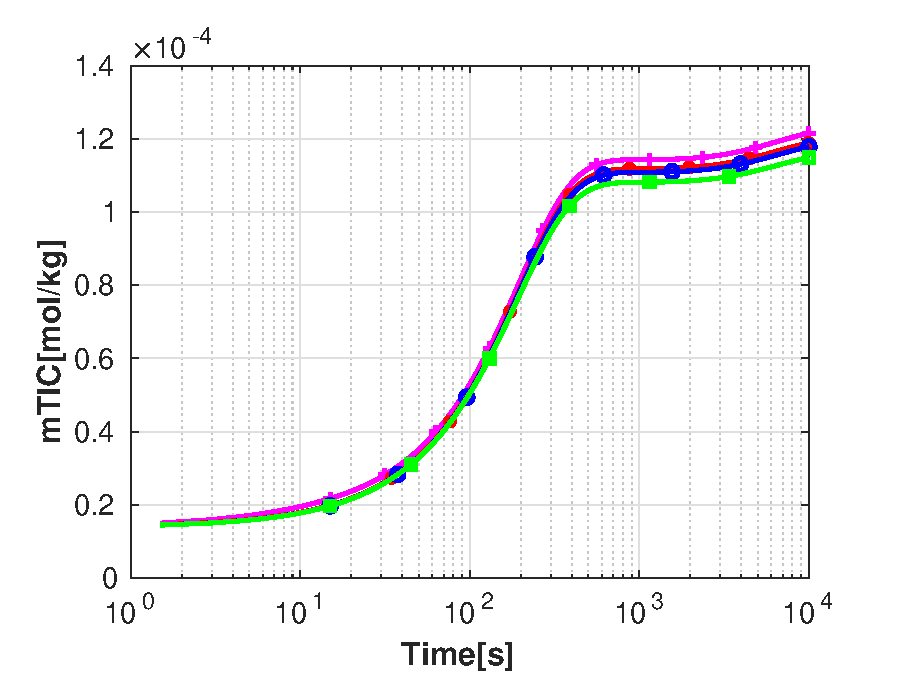
\includegraphics[width=\textwidth]{PICTURES/without_pH_mTIC.eps}
        \caption{Change in molality of total inorganic carbon (mTIC)}
        \label{fig:withoutpHmTIC}
    \end{subfigure}%
    \hfill
    \begin{subfigure}{.5\linewidth}
            \centering
        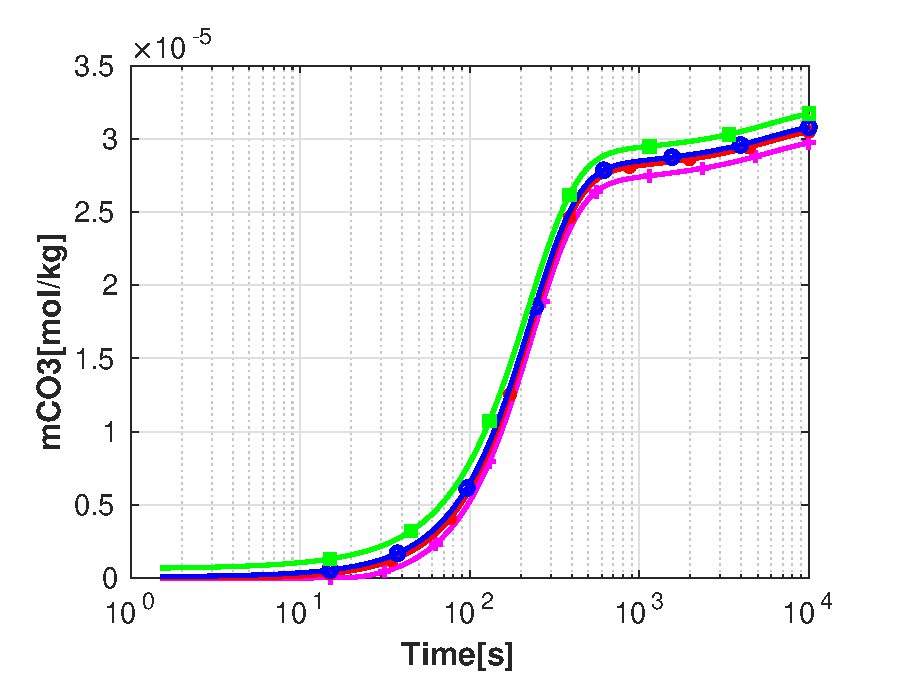
\includegraphics[width=\textwidth]{PICTURES/without_pH_mCO3.eps}
        \caption{Change in molality of carbonate (mCO3)}
        \label{fig:withoutpHmCO3}
    \end{subfigure}%
    \hfill
    \begin{subfigure}{.5\linewidth}
            \centering
        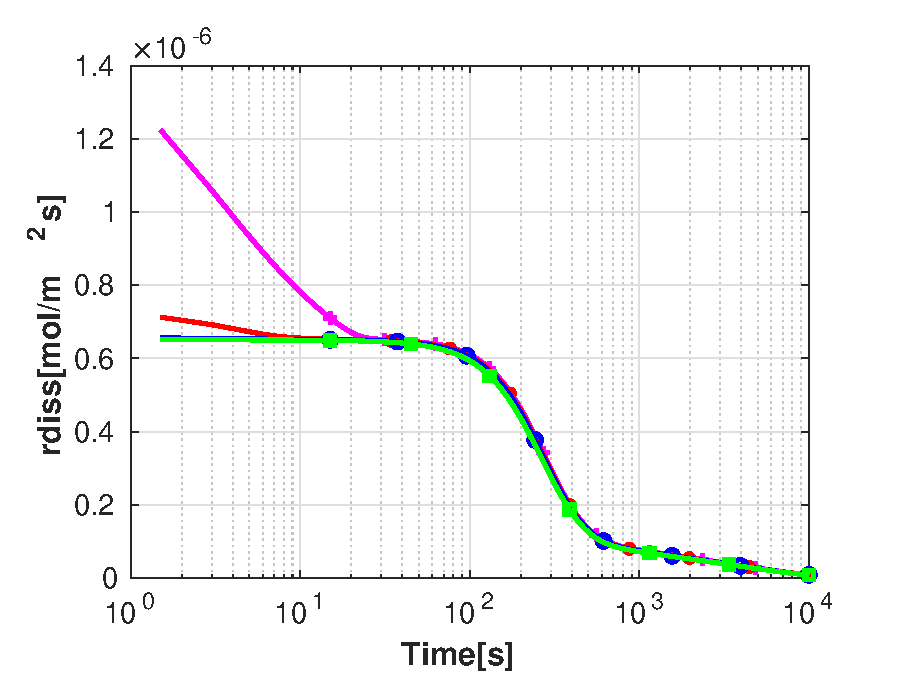
\includegraphics[width=\textwidth]{PICTURES/without_pH_rdiss.eps}
        \caption{Change in rate of dissolution of calcite (rdiss)}
        \label{fig:withoutpHrdiss}
    \end{subfigure}%
  \hfill
  \begin{subfigure}{.5\linewidth}
            \centering
        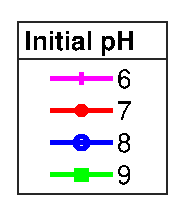
\includegraphics[width=0.25\textwidth]{PICTURES/with_pH_legend.eps}
        \caption{Legend}
        \label{fig:withoutpHlegend}
    \end{subfigure}%
    \caption{\DuMuX results that show the change in pH (\cref{fig:withoutpHpH}), molality of calcium (\cref{fig:withoutpHmCa}), molality of total inorganic carbon (\cref{fig:withoutpHmTIC}), molality of carbonate (\cref{fig:withoutpHmCO3}) and rate of dissolution of calcite (\cref{fig:withoutpHrdiss}) in time for different initial pH in a closed system}
    
    \label{fig:comparisionWithoutDiffInitialpH}
\end{figure}

The figure \ref{fig:diffInitialpHNoFlow}, for all the sub-plots, shows pH increases as the dissolution advances and after some time it reaches steady-state condition. Unlike a similar scenario with flow-velocity, as shown in figure \ref{fig:comparisionDiffInitialpH}, there is no descend curve. The reasons are: there is no flow-velocity to transport the dissolved calcium-carbonate out of the system, and the karst water is not in contact with the outer environment, hence there is no transport of TIC into the karst water, which means there is no rapid increase in pH and no descend curve, rather pH increases constructively and stabilizes to a steady-state value.


\subsubsection*{Different Grid grading parameter} \label{ssec:diffGridnoflow}
We fixed the initial pH in the karst water to 6.0 and the initial concentration of \ce{CO2}  was set to 2.5e-7 [mol/mol]. We decreased the spacing of the grids near the wall in x-direction. We ran the simulation for grid-grading values 1.1 and 1.2. 

\begin{figure}[!h]
        \centering
    \begin{subfigure}{.5\linewidth}
            \centering
        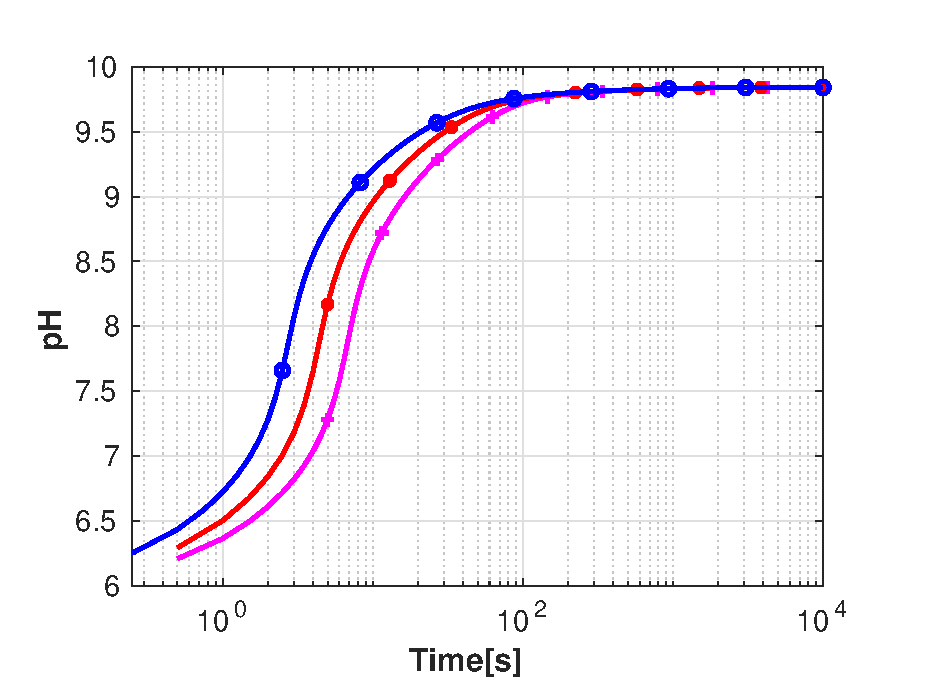
\includegraphics[width=\textwidth]{PICTURES/without_grid_pH.eps}
        \caption{Change in pH}
        \label{fig:withoutgridpH}
    \end{subfigure}%
        \hfill
    \begin{subfigure}{.5\linewidth}
            \centering
        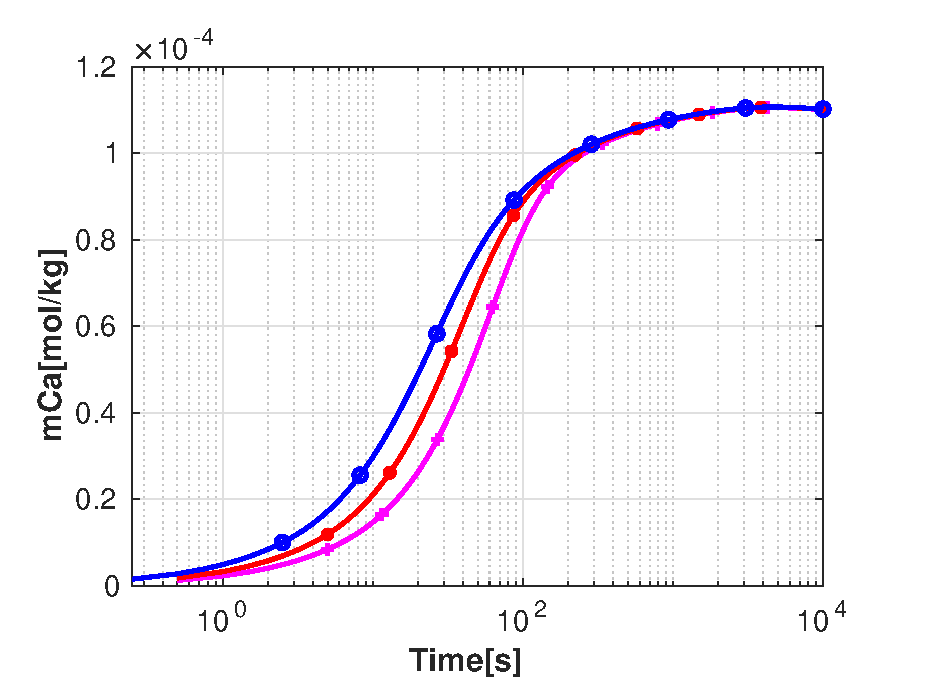
\includegraphics[width=\textwidth]{PICTURES/without_grid_mCa.eps}
        \caption{Change in molality of calcium (mCa)}
        \label{fig:withoutgridmCa}
    \end{subfigure}%
    \hfill
    \begin{subfigure}{.5\linewidth}
            \centering
        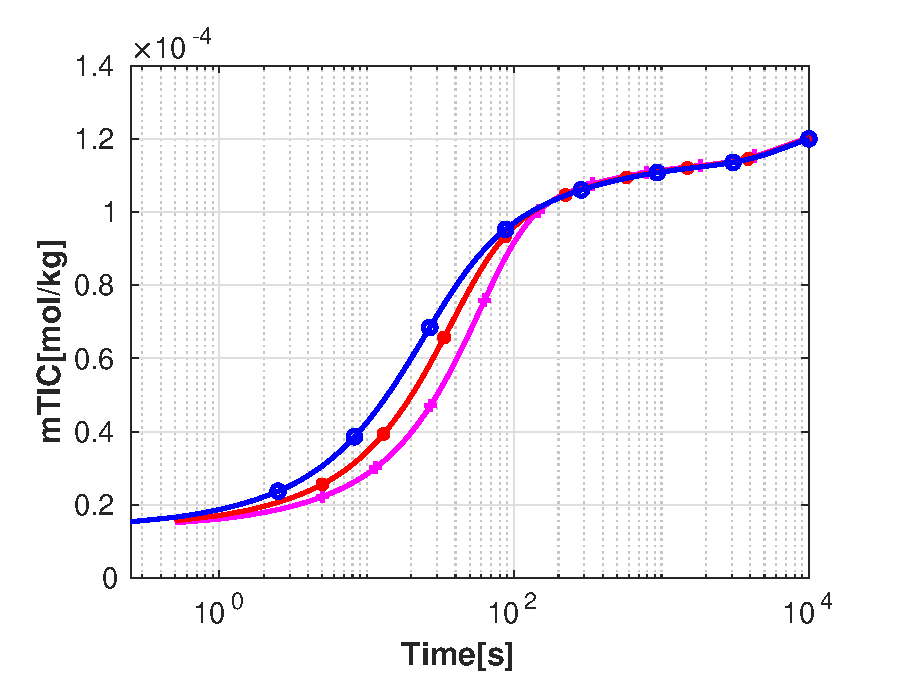
\includegraphics[width=\textwidth]{PICTURES/without_grid_mTIC.eps}
        \caption{Change in molality of total inorganic carbon (mTIC)}
        \label{fig:withoutgridmTIC}
    \end{subfigure}%
    \hfill
    \begin{subfigure}{.5\linewidth}
            \centering
        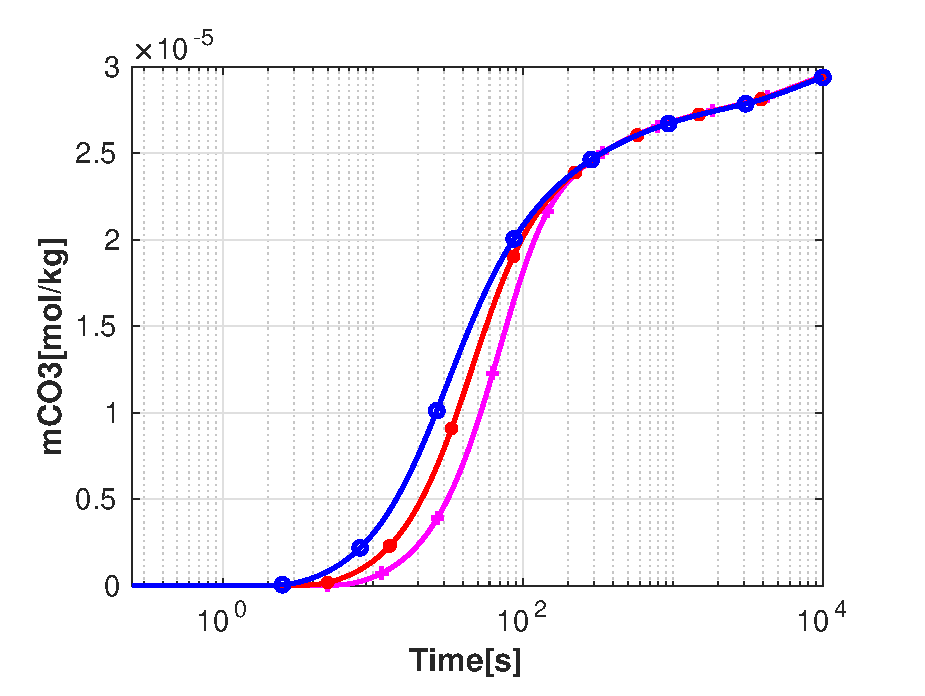
\includegraphics[width=\textwidth]{PICTURES/without_grid_mCO3.eps}
        \caption{Change in molality of carbonate (mCO3)}
        \label{fig:withoutgridmCO3}
    \end{subfigure}%
    \hfill
    \begin{subfigure}{.5\linewidth}
            \centering
        \includegraphics[width=\textwidth]{PICTURES/without_grid_rdiss.eps}
        \caption{Change in rate of dissolution of calcite (rdiss)}
        \label{fig:withoutgridrdiss}
    \end{subfigure}%
  \hfill
  \begin{subfigure}{.5\linewidth}
            \centering
        \includegraphics[width=0.35\textwidth]{PICTURES/with_grid_legend.eps}
        \caption{Legend}
        \label{fig:withoutgridlegend}
    \end{subfigure}%
    \caption{\DuMuX results that show the change in pH (\cref{fig:withoutgridpH}), molality of calcium (\cref{fig:withoutgridmCa}), molality of total inorganic carbon (\cref{fig:withoutgridmTIC}), molality of carbonate (\cref{fig:withoutgridmCO3}) and rate of dissolution of calcite (\cref{fig:withoutgridrdiss}) in time for different grid grading parameter in a closed system} 
    \label{fig:comparisionWithoutDiffgrid}
\end{figure}

The sub-figures \subref{fig:Noflowgrid1.1} and \subref{fig:Noflowgrid1.2} in the figure \ref{ssec:diffGridnoflow} did not show any differences. The reason is the same as explained in subsection \ref{ssec:diffGrid}.

\section{\MATLAB Simulation results}
\MATLAB Simulation results for a closed system. 

\begin{figure}[!h]
        \centering
    \begin{subfigure}{.5\linewidth}
        \centering
        \includegraphics[width=\textwidth]{PICTURES/without_vel_pH.eps}
        \caption{Change in pH}
        \label{fig:withoutvelpH}       % Give a unique label
    \end{subfigure}%
        \hfill
        % here was an empty line which caused that the plots where not next
        % to each other but on top of each other
    \begin{subfigure}{.5\linewidth}
        \centering
        \includegraphics[width=\textwidth]{PICTURES/without_vel_mCa.eps}
        \caption{Change in molality of calcium (mCa)}
        \label{fig:withoutvelmCa}       % Give a unique label
    \end{subfigure}%
        \hfill
    \begin{subfigure}{.5\linewidth}
        \centering
        \includegraphics[width=\textwidth]{PICTURES/without_vel_mTIC.eps}
        \caption{Change in molality of total inorganic carbon (mTIC)}
        \label{fig:withoutvelmTIC}
    \end{subfigure}%
    \hfill
    \begin{subfigure}{.5\linewidth}
        \centering
        \includegraphics[width=\textwidth]{PICTURES/without_vel_mCO3.eps}
        \caption{Change in molality of carbonate (mCO3)}
        \label{fig:withoutvelmCO3}
    \end{subfigure}%
    \hfill
    \begin{subfigure}{.5\linewidth}
        \centering
        \includegraphics[width=\textwidth]{PICTURES/without_vel_rdiss.eps}
        \caption{Change in rate of dissolution of calcite (rdiss)}
        \label{fig:withoutvelrdiss}
    \end{subfigure}%
    \hfill
    \begin{subfigure}{.5\linewidth}
        \centering
        \includegraphics[width=0.25\textwidth]{PICTURES/with_pH_legend.eps}
        \caption{Legend}
        \label{fig:withoutvellegend}
    \end{subfigure}%
     \caption{\MATLAB results that show the change in pH (\cref{fig:withoutvelpH}), molality of calcium (\cref{fig:withoutvelmCa}), molality of total inorganic carbon (\cref{fig:withoutvelmTIC}), molality of carbonate (\cref{fig:withoutvelmCO3}) and rate of dissolution of calcite (\cref{fig:withoutvelrdiss}) in time for different initial pH in a closed system of 2D volume [15mm $\times$ 5mm]}
     \label{fig:MATLABcomparisionDiffInitialpH}
\end{figure}


\section{Comparison \DuMuX and \MATLAB} \label{sec:dvm}
A comparision between \MATLAB and \DuMuX is presented in this section. 
\begin{table}[ht]
\small\addtolength{\tabcolsep}{-12pt}
\centering
\caption{\DuMuX and \MATLAB comparison table that lists steady-state time, pH, molality of calcium (mCa), molality of total inorganic carbon (mTIC) and molality of carbonate (mCO3) for a closed system of size 15mm$\times$5mm with varying initial pH, reactive area and batch volume}
\begin{tabular}{|c|c|c|c|c|c|c|c|c|c|c|c|c|}
    \hline
    \thead{Initial \\pH} & \thead{Reactive \\area} & \thead{Batch \\Volume} & \multicolumn{5}{c|}{\thead{Steady-state \MATLAB}} & \multicolumn{5}{c|}{\thead{Steady-state \DuMuX}} \\
    \cline{4-13}
    & & & \thead{time} & \thead{pH} & \thead{mCa}      & \thead{mTIC}     & \thead{mCO3}     & \thead{time} & \thead{pH} & \thead{mCa}      & \thead{mTIC}     & \thead{mCO3}\\
    & mm & \ce{mm^2} &  [s]  & [-] & [mol/kg] & [mol/kg] & [mol/kg] & [s] & [-]   & [mol/kg] & [mol/kg] & [mol/kg]\\
    \hline
    % initial pH   Reactive area Batch Volume time pH mCa mTIC mCO3 time pH mCa mTIC mCO3
      & 5  & 5   & 321  & 9.83 & 1.09e-4 & 1.23e-4 & 3.01e-5 & 321 & 9.83 & 1.09e-4 & 1.23e-4 & 3.01e-5 \\
    6 & 15 & 75  & 1601 & 9.83 & 1.09e-4 & 1.23e-4 & 3.01e-5 & 1596 & 9.83 & 1.09e-4 & 1.23e-4 & 3.01e-5 \\
      & 30 & 300 & 3201 & 9.83 & 1.09e-4 & 1.23e-4 & 3.01e-5 & 3190 & 9.83 & 1.09e-4 & 1.23e-4 & 3.01e-5 \\
    \hline
      & 5  & 5   & 331  & 9.86 & 1.06e-4 & 1.20e-4 & 3.09e-5 & 338  & 9.86 & 1.06e-4 & 1.20e-4 & 3.09e-5 \\
    7 & 15 & 75  & 1701 & 9.86 & 1.06e-4 & 1.20e-4 & 3.09e-5 & 1679 & 9.86 & 1.06e-4 & 1.20e-4 & 3.09e-5 \\
      & 30 & 300 & 3301 & 9.86 & 1.06e-4 & 1.20e-4 & 3.09e-5 & 3357 & 9.86 & 1.06e-4 & 1.20e-4 & 3.09e-5 \\
    \hline
      & 5  & 5   & 321  & 9.87 & 1.05e-4 & 1.19e-4 & 3.12e-5 & 324  & 9.87 & 1.05e-4 & 1.19e-4 & 3.12e-5 \\
    8 & 15 & 75  & 1701 & 9.87 & 1.05e-4 & 1.19e-4 & 3.12e-5 & 1610 & 9.87 & 1.05e-4 & 1.19e-4 & 3.12e-5 \\
      & 30 & 300 & 3201 & 9.87 & 1.05e-4 & 1.19e-4 & 3.12e-5 & 3219 & 9.87 & 1.05e-4 & 1.19e-4 & 3.12e-5 \\
    \hline
      & 5  & 5   & 611  & 9.91 & 1.02e-4 & 1.16e-4 & 3.21e-5 & 294  & 9.90 & 1.02e-4 & 1.16e-4 & 3.21e-5 \\
    9 & 15 & 75  & 3001 & 9.91 & 1.02e-4 & 1.16e-4 & 3.21e-5 & 1463 & 9.90 & 1.02e-4 & 1.16e-4 & 3.21e-5 \\
      & 30 & 300 & 6101 & 9.91 & 1.02e-4 & 1.16e-4 & 3.21e-5 & 2924 & 9.90 & 1.02e-4 & 1.16e-4 & 3.21e-5 \\
    \hline
\end{tabular}
% \end{adjustbox}
\label{tab:DumuxVsMatlab}
\end{table}


\begin{figure}[!h]
        \centering
    \begin{subfigure}{.5\linewidth}
            \centering
        \includegraphics[width=\textwidth]{PICTURES/dvm_pH6_pH.eps}
        \caption{Change in pH}
        \label{fig:dvmpH6pH}
    \end{subfigure}%
        \hfill
    \begin{subfigure}{.5\linewidth}
            \centering
        \includegraphics[width=\textwidth]{PICTURES/dvm_pH6_mCa.eps}
        \caption{Change in molality of calcium (mCa)}
        \label{fig:dvmpH6mCa}
    \end{subfigure}%
    \hfill
    \begin{subfigure}{.5\linewidth}
            \centering
        \includegraphics[width=\textwidth]{PICTURES/dvm_pH6_mTIC.eps}
        \caption{Change in molality of total inorganic carbon (mTIC)}
        \label{fig:dvmpH6mTIC}
    \end{subfigure}%
    \hfill
    \begin{subfigure}{.5\linewidth}
            \centering
        \includegraphics[width=\textwidth]{PICTURES/dvm_pH6_mCO3.eps}
        \caption{Change in molality of carbonate (mCO3)}
        \label{fig:dvmpH6mCO3}
    \end{subfigure}%
    \hfill
    \begin{subfigure}{.5\linewidth}
            \centering
        \includegraphics[width=\textwidth]{PICTURES/dvm_pH6_rdiss.eps}
        \caption{Change in rate of dissolution of calcite (rdiss)}
        \label{fig:dvmpH6rdiss}
    \end{subfigure}%
  \hfill
  \hfill
    \begin{subfigure}{.5\linewidth}
            \centering
        \includegraphics[width=0.85\textwidth]{PICTURES/dvm_pH6_legend.eps}
        \caption{Legend}
        \label{fig:dvmpH6legend}
    \end{subfigure}%
    \caption{Comparison: \DuMuX and \MATLAB results that show the change in pH (\cref{fig:dvmpH6pH}), molality of calcium (\cref{fig:dvmpH6mCa}), molality of total inorganic carbon (\cref{fig:dvmpH6mTIC}), molality of carbonate (\cref{fig:dvmpH6mCO3}) and rate of dissolution of calcite (\cref{fig:dvmpH6rdiss}) in time for initial pH 6.0 in a closed system of 2D volume [15mm $\times$ 5mm]} 
    \label{fig:comparisionDumuxMatlab_pH6.0}
\end{figure}

\endinput